\documentclass[a4paper,11pt]{article}
\usepackage[margin=20mm]{geometry}
\usepackage{graphicx,booktabs,hyperref}
\begin{document}
\title{PM12 channel 12: integrator balance and signed ramp response}
\author{FIT hardware acceptance bench}\date{13 November 2026}\maketitle
\section{Setup and controls}
PM12 FPGA DNA 3A17A1B402212223 was established in the previous restoration;
MCU EEPROM serial 1803, the resident FPGA identity and physical PGOOD were
checked for these measurements. Original INTA/INTB CPLD12 gates were restored
and vendor-verified on 12 November. Today's Kasli preflight observed 683/682
rising edges on INTA/INTB. No clock profile or FPGA/CPLD image was changed.

The owner moved the MOD-DAC-28 USB cable from the direct ADC injection input
J8 to the integrator stimulus input J6. CH0/CH1 are controlled through the
existing SCPI entities; instrument identity FIT-CTRL-6825DD4C49E4 is checked.
Every command is limited to 0--3.3 V per output. The shared local and station2
leases cover the complete hardware session. Other DAC outputs are unchanged.

CFD MCP23017: GPA7 LOW releases Integrator\_PDn and enables the amplifiers;
GPB5 HIGH isolates the direct-ADC injection mux. GPA3 HIGH keeps the monitor
output inhibited. GPIO latches and directions are checked by readback.

The initial assumed 1.024/2.048 V input order saturated both ADCs at code 0.
A mapping scan found a usable region with the reverse DAC coordinate order.
The working coordinate system is therefore
\[ V_{CH0}=2.048\,\mathrm V+\delta/2,\qquad
   V_{CH1}=1.024\,\mathrm V-\delta/2. \]
The actual differential setpoint is $1.024\,\mathrm V+\delta$.
This is an empirically established fixture coordinate system, not an independent
measurement of adapter polarity or board reference voltages.
\section{Method}
Integrators remain at nominal 20 MHz and ADCs at nominal 80 MHz: four ADC samples
per integration/reset cycle. For each setting, frozen 4096-word FPGA buffers
are downloaded over IPbus and strobe-decimated with timing/coherency validation.
The coarse scan has 13 settings; the fine scan has 26 settings from $-12$ to
$-2$ mV in 0.4 mV steps, with four buffers per ADC/setting.

Capture start is not tagged with integrator phase. Within each buffer, the
separated four-phase template is aligned to its highest adjacent pair, assigned
to integration by its strong input-dependent ramp response. The observable is
late minus early ADC code, averaged over approximately 255 cycles/buffer.
Clipped traces and ambiguous templates are rejected; a saturated constant output
is never classified as balance. Thirty-two coarse buffers were rejected.
\clearpage
\section{Zero crossings and response}
\begin{center}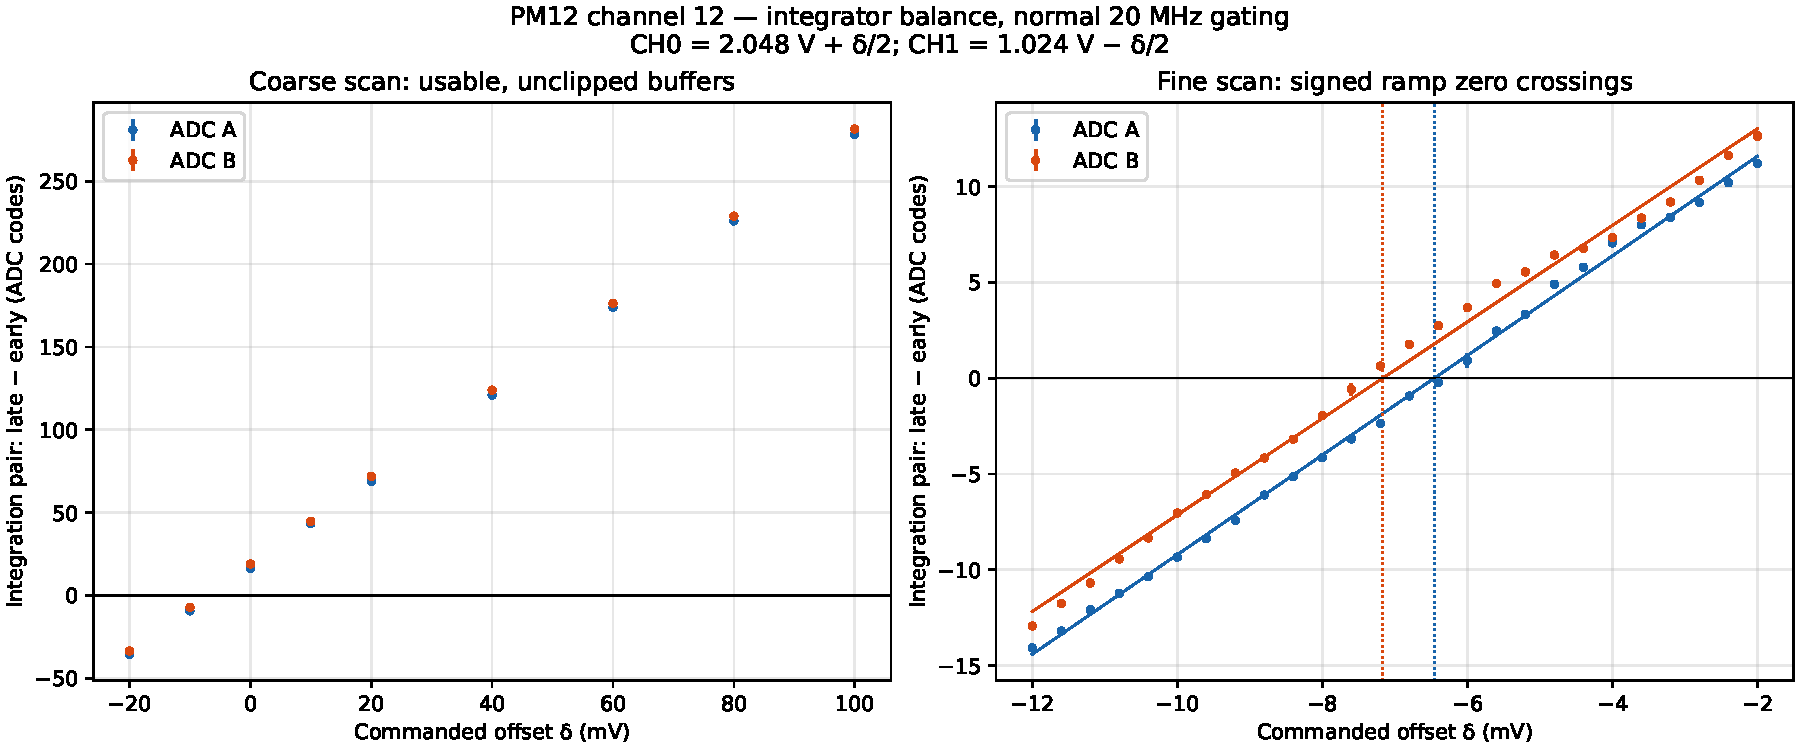
\includegraphics[width=\textwidth]{integrator-balance.pdf}\end{center}
\begin{center}\begin{tabular}{r rrr r}\toprule
ADC & Local zero $\delta$ (mV) & CH0 (V) & CH1 (V) & Gain (codes/V)\\\midrule
A & -6.319 & 2.044840 & 1.027160 & 2599.6 \\
B & -7.411 & 2.044295 & 1.027705 & 2520.0 \\
\bottomrule\end{tabular}\end{center}
Zeros in the table are local interpolation of adjacent sign-changing fine-scan
points. Gain is a linear fit to the full fine scan. Global fit residual RMS is
0.318/0.550 codes (A/B). Fit-only statistical uncertainties exclude DAC
quantization, voltage accuracy, timing calibration and drift.
\section{Independent returns to the operating points}
The validation sequence revisited each operating point, measured both ADCs,
and applied positive and negative 5 mV differential offsets. Each retained setting
uses eight buffers, approximately 2040 cycles per ADC; the final candidate points
were revisited twice. The observed near-zero changes were:
\begin{center}\begin{tabular}{r rrr}\toprule
ADC & Tested CH0 (V) & Tested CH1 (V) & Change (codes/ADC interval)\\\midrule
A & 2.0448 & 1.0272 & -0.281 \\
B & 2.0443 & 1.0277 & +0.329 \\
\bottomrule\end{tabular}\end{center}
The $\pm5$ mV offsets produce approximately $\pm13$ codes of change, with opposite
signs. The two A/B balance points differ: one shared stimulus cannot null both
exactly. A compromise setting is retained rather than declaring both perfectly flat.
\clearpage
\section{Captured waveforms}
\begin{center}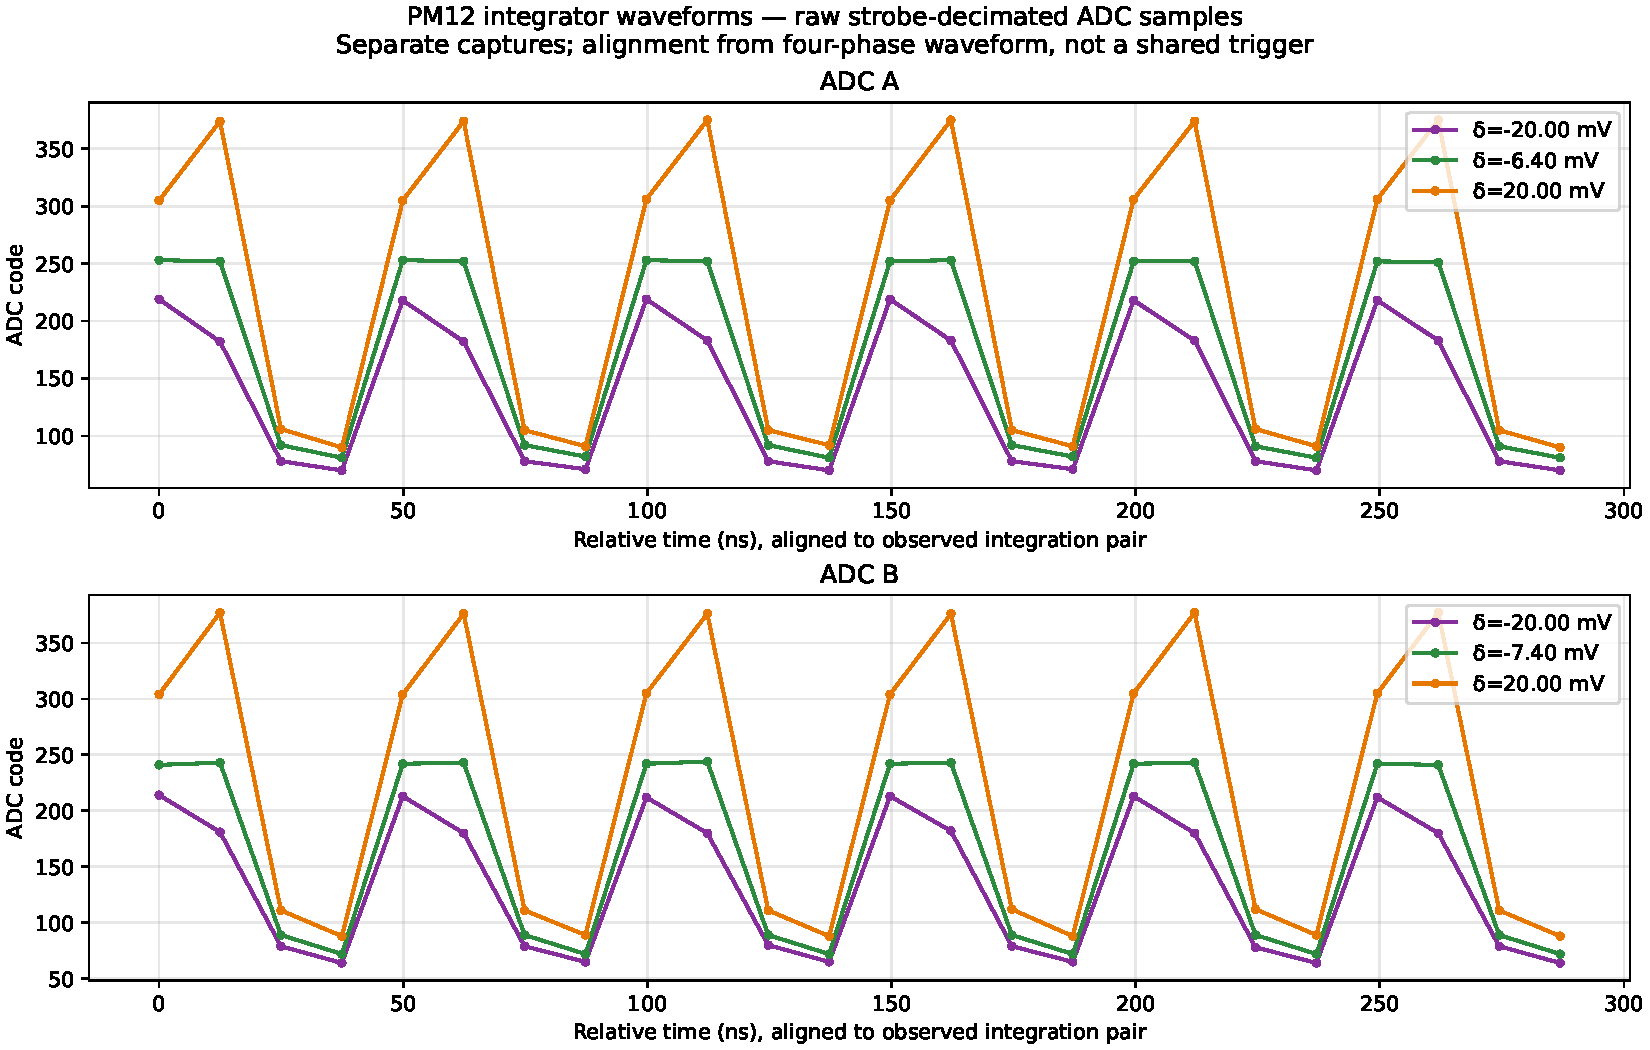
\includegraphics[width=\textwidth]{integrator-waveforms.pdf}\end{center}
Each trace is aligned locally, without an external trigger epoch. Timing assumes
an ADC rate of 80.1574 MS/s from a 40.0787 MHz reference. No frequency counter
check was made. Two adjacent samples are about 12.475 ns apart. A zero change
applies to the selected integration samples; reset steps remain.
\section{Final state and limits}
Amplifiers remain enabled, direct ADC bypass isolated, monitor inhibited and
both upstream TCA masks disconnected. DAC CH0/CH1 are parked at
2.0446/1.0274 V, between the measured A/B zero points. Other outputs are unchanged.
The last capture is ADC A. No firmware, clock, EEPROM or configuration-flash
write was needed.

These are whole DAC/cable/integrator/ADC-chain results against commanded
voltages. They establish a signed response and an effective differential balance
point, not separately measured input bias of each opamp, calibrated capacitor
value, resolved intra-sample curvature, or intrinsic jitter/noise.
Raw buffers, rejected probes, command receipts and analysis hashes are retained.
\end{document}
